% AI-assisted working draft for team review, not an approved final section.
% Requires amsmath, graphicx and booktabs. Merge references.bib into the report bibliography.
\section{Simple square demonstration}
\label{sec:square}

We now apply the construction of Section~\ref{sec:mechanics-matrix} and the
protocol of Section~\ref{sec:solvers} to the simplest controlled case: a
square plate pulled uniformly at one end, whose expected stretch $pL/E$
lets us check every computed number against physics.

The plate occupies $0\le x,y\le L$ with $L=1$~m and has thickness
$t=0.01$~m, $E=200$~GPa and $\nu=0.3$, in plane stress without body forces
(Fig.~\ref{fig:square-setup}a). The left edge is clamped, $u_x=u_y=0$. The
right edge carries the uniform traction $\bar\tau=(p,0)$ with $p=100$~MPa,
so $q=tp=10^6$~N/m with resultant $ptL=10^6$~N; the top and bottom edges
are free; the load is a prescribed traction, not a prescribed
displacement. Units are m, Pa and N. The mesh has $m\times m$ square cells,
each cut along its bottom-left to top-right diagonal, giving $(m+1)^2$
nodes and $2m^2$ triangles. The clamp prescribes $2(m+1)$ components,
leaving $N=2m(m+1)$ unknowns. The case is \texttt{force\_driven} in
\texttt{fem/plate.py}; all numbers below come from
\texttt{draft/experiments/square.py}.

\begin{figure}[htbp]
 \centering
 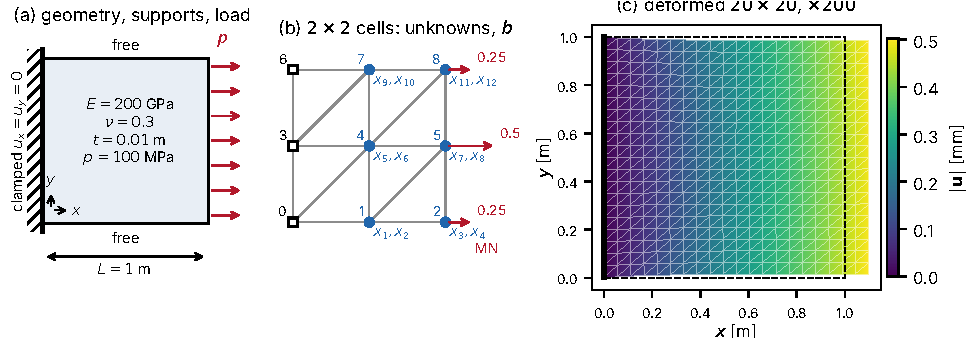
\includegraphics[width=\linewidth]{figures/square_setup.pdf}
 \caption{(a) Geometry, supports and load. (b) The $2\times2$-cell mesh:
 clamped nodes (squares), free nodes (dots) with their unknowns
 $x_1,\dots,x_{12}$, and the nodal forces forming $b$. (c) Original outline
 (dashed) and deformed $20\times20$-cell plate, displacements amplified by
 200; colour is the actual displacement magnitude in mm.}
 \label{fig:square-setup}
\end{figure}

\subsection{A small system solved directly}
For $m=2$ there are 9 nodes, 8 triangles and 18 displacement components.
Clamping nodes 0, 3 and 6 leaves $N=12$ unknowns, ordered node by node as
$x=(u_{x,1},u_{y,1},u_{x,2},\dots,u_{y,8})^T$
(Fig.~\ref{fig:square-setup}b). Since $d_C=0$, $b=f_F$. Each loaded edge of
length $0.5$~m carries $0.5$~MN, split equally between its end nodes, so
$b=2.5\times10^5\,(0,0,1,0,0,0,2,0,0,0,1,0)^T$~N. For $\nu=0.3$ every entry
of $A$ is an integer multiple of $Et/(40(1-\nu^2))=5.495\times10^7$~N/m:
\begin{equation}
 \setlength{\arraycolsep}{3.2pt}
 A=\frac{Et}{40(1-\nu^2)}\scriptsize
 \left[\begin{array}{@{}*{12}{r}@{}}
 54 & -13 & -20 & 6 & -14 & 13 & \cdot & -13 & \cdot & \cdot & \cdot & \cdot \\
 -13 & 54 & 7 & -7 & 13 & -40 & -13 & \cdot & \cdot & \cdot & \cdot & \cdot \\
 -20 & 7 & 27 & -13 & \cdot & \cdot & -7 & 6 & \cdot & \cdot & \cdot & \cdot \\
 6 & -7 & -13 & 27 & \cdot & \cdot & 7 & -20 & \cdot & \cdot & \cdot & \cdot \\
 -14 & 13 & \cdot & \cdot & 108 & -26 & -40 & 13 & -14 & 13 & \cdot & -13 \\
 13 & -40 & \cdot & \cdot & -26 & 108 & 13 & -14 & 13 & -40 & -13 & \cdot \\
 \cdot & -13 & -7 & 7 & -40 & 13 & 54 & -13 & \cdot & \cdot & -7 & 6 \\
 -13 & \cdot & 6 & -20 & 13 & -14 & -13 & 54 & \cdot & \cdot & 7 & -20 \\
 \cdot & \cdot & \cdot & \cdot & -14 & 13 & \cdot & \cdot & 54 & -13 & -20 & 7 \\
 \cdot & \cdot & \cdot & \cdot & 13 & -40 & \cdot & \cdot & -13 & 54 & 6 & -7 \\
 \cdot & \cdot & \cdot & \cdot & \cdot & -13 & -7 & 7 & -20 & 6 & 27 & \cdot \\
 \cdot & \cdot & \cdot & \cdot & -13 & \cdot & 6 & -20 & 7 & -7 & \cdot & 27
 \end{array}\right].
 \label{eq:square-small-matrix}
\end{equation}
Dots are zeros, mostly between nodes without a common triangle, such as 1
and 7. $A$ is exactly symmetric, with eigenvalues from $\lambda_{\min}=1.073\times10^8$ to
$\lambda_{\max}=1.028\times10^{10}$~N/m, so $\kappa_2(A)=95.80$; the
arrays are stored as CSV files in \texttt{draft/experiments/results/square/}.

Pivoted $PA=LU$, the explicit inverse and Cholesky $A=LL^T$ give relative
residuals $\eta$ (Eq.~\eqref{eq:solvers-residual}) of $6.2\times10^{-16}$,
$8.4\times10^{-16}$ and $9.2\times10^{-16}$, and their solutions agree to
$6.3\times10^{-16}$ relative to their norm. From bottom to top, the
right-edge nodes move $u_x=0.5112$, $0.4822$ and $0.4678$~mm, close to
$pL/E=0.5$~mm, and $u_y=+0.1045$, $+0.0294$ and $-0.0461$~mm. The continuum
problem is symmetric about $y=L/2$, which would make $u_y$ antisymmetric;
the deviation comes from the coarse mesh and its single diagonal direction.

\subsection{A larger system and the iterative methods}
For $m=20$ the mesh has 441 nodes, 800 triangles and $N=840$ unknowns. The
sparse matrix stores 11{,}112 entries (9{,}590 numerically nonzero) and is
symmetric up to rounding. Sparse estimates give $\lambda_{\min}=1.917\times10^6$ and
$\lambda_{\max}=1.745\times10^{10}$~N/m, so $\kappa_2(A)=9104$, in agreement
with a dense computation to $10^{-14}$. The scaled matrix $S$ has
eigenvalues in $[3.687\times10^{-4},\,2.960]$, so
$\rho_J=1.960$ by Eq.~\eqref{eq:solvers-jacobi-radius}.
Table~\ref{tab:square-solvers} and Fig.~\ref{fig:square-residuals} report
the methods.

\begin{table}[htbp]
 \centering
 \caption{All methods on the 840-unknown system under the protocol of
 Section~\ref{sec:solvers} (best of three times; Linux x86-64, Python 3.13,
 SciPy 1.18.1). An asterisk marks failure to reach $\eta<10^{-8}$.}
 \label{tab:square-solvers}
 \small
 \begin{tabular}{@{}lrrrrl@{}}
 \toprule
 Method & Iterations & Final $\eta$ & Error vs LU & Time (ms) & Stop \\
 \midrule
 Sparse LU (\texttt{splu}) & -- & $3.5\times10^{-14}$ & -- & $2.12+0.09$ & factor + solve \\
 Jacobi* & 49 & $1.3\times10^{10}$ & $3.4\times10^{7}$ & 0.78 & divergence guard \\
 Damped Jacobi ($\omega=0.5$)* & 20{,}000 & $4.8\times10^{-6}$ & $8.7\times10^{-5}$ & 246 & iteration cap \\
 Gauss--Seidel & 19{,}136 & $1.0\times10^{-8}$ & $1.7\times10^{-7}$ & 7{,}437 & target \\
 Steepest descent* & 20{,}000 & $3.1\times10^{-6}$ & $4.2\times10^{-5}$ & 532 & iteration cap \\
 CG & 242 & $8.8\times10^{-9}$ & $9.6\times10^{-10}$ & 5.3 & target \\
 Diagonal PCG & 226 & $8.8\times10^{-9}$ & $4.9\times10^{-10}$ & 5.3 & target \\
 MINRES & 236 & $9.4\times10^{-9}$ & $5.9\times10^{-9}$ & 11.0 & target \\
 Full GMRES ($\text{restart}=N$) & 228 & $9.5\times10^{-9}$ & $6.0\times10^{-9}$ & 150 & target \\
 \bottomrule
 \end{tabular}
\end{table}

\begin{figure}[htbp]
 \centering
 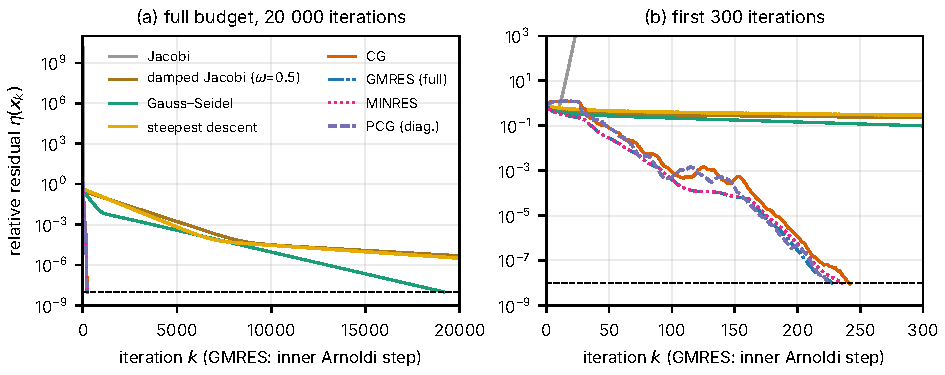
\includegraphics[width=\linewidth]{figures/square_residuals.pdf}
 \caption{Relative residual $\eta(x_k)$ of every method on the
 840-unknown system; the dashed line is the target $10^{-8}$. (a) Whole
 budget. (b) First 300 iterations. GMRES shows its Arnoldi residual
 estimate; other curves are recomputed residuals.}
 \label{fig:square-residuals}
\end{figure}

The stationary methods behave as their diagnostics predict. Since
$\lambda_{\max}(S)>2$, Jacobi multiplies one error component by about
$-1.96$ per sweep and is stopped by the guard after 49 sweeps. Damping
with $\omega=0.5$, below the limit $2/\lambda_{\max}(S)=0.676$, restores
convergence, but the slowest component shrinks only by
$1-\omega\lambda_{\min}(S)=0.99982$ per sweep, a factor of $0.025$ over the
whole budget. Steepest descent is limited similarly: at most
$(\kappa-1)/(\kappa+1)$ per step gives about $0.012$ over 20{,}000 steps.
Gauss--Seidel meets the target after 19{,}136 sweeps; its long time mainly
reflects one sparse triangular solve per sweep in this implementation.

The Krylov methods need 226--242 iterations. Bound
\eqref{eq:solvers-cg-bound} guarantees an energy-norm reduction by
$10^{-8}$ within $\tfrac12\sqrt{\kappa}\ln(2\times10^8)\approx912$ CG
iterations; CG needs about a quarter of this, because the bound uses only
the extreme eigenvalues~\cite{shewchuk-cg}. Diagonal preconditioning helps little:
$\kappa_2(S)=8029$ is only 12\% below $\kappa_2(A)$, since the diagonal of
$A$ varies only near the boundary, and PCG saves 16 iterations. Full GMRES
needs the fewest iterations but is 28 times slower than CG, the cost of
orthogonalizing against all previous basis vectors~\cite{saad-iterative}. At this size, sparse
LU factorization and solve together take 2.2~ms, less than any iterative
method.

Equal residual targets do not give equal accuracy: the errors of
Gauss--Seidel and CG differ by a factor of 180, both within the bound $\kappa_2(A)\,\eta\approx9.1\times10^{-5}$ from
Eq.~\eqref{eq:solvers-perturbation}. Iterations are algebraic corrections
towards one static equilibrium, not physical time steps.

\subsection{Deformation and validation}
Figure~\ref{fig:square-setup}c shows the $20\times20$ solution. The right
edge moves between $0.4916$~mm (mid-height) and $0.4967$~mm (bottom
corner), close to $pL/E=0.5$~mm. Near the loaded end, the top and bottom
edges move inwards by $0.077$ and $0.079$~mm, together matching the free
lateral contraction $\nu pL/E=0.15$~mm. The clamp prevents this
contraction at $x=0$, producing the tapered shape.

We check this solution in three ways. All 42 prescribed components are
exactly zero in the reconstructed $d$. The reactions of
Eq.~\eqref{eq:mechanics-reactions} sum to $-1.000\times10^6$~N in $x$,
leaving a force imbalance of $(-4.0,-2.6)\times10^{-9}$~N and a moment
imbalance about the origin of $4.5\times10^{-9}$~N\,m, against an applied
moment of $5\times10^5$~N\,m. The five methods that met the target agree
with LU to at most $1.7\times10^{-7}$ relative, or $8.3\times10^{-8}$~mm in
any component. On the same mesh, the roller-supported patch test of
Section~\ref{sec:solvers} (860 unknowns) reproduces the exact field
$u_x=px/E$, $u_y=-\nu py/E$ with relative error $2.6\times10^{-14}$,
verifying assembly, loading and reduction. The clamped plate has no
closed-form solution, so Section~\ref{sec:results} estimates its
discretization error by comparing meshes from $5\times5$ to $80\times80$
cells, together with the growth of $\kappa_2(A)$ and the iteration counts.
